\Section{Implementation in the energy extraction algorithm}

\par As seen in the previous chapter the optimization process for the energy extraction trajectory only requires a way to calculate the relationship between the lift and drag coefficient.
In our case these two variables depend only on the angle of attack and its change rate over time, it is fairly easy to implement it into the algorithm.
However the non-dimensional time constants are different for fluid dynamics and vehicle dynamics.
The energy extraction one considers the optimal glide speed and the gravity acceleration, whereas the one used for the GK model uses the flight speed and the chord length.

\Subsection{Relation between the different time scales}
As said before the time scale used in the two models are different.
To solve this issue the ratio of the two time constants are plotted (see figure \ref{fig:T_t+_ratio}) for a wide variety of flying objects.

\begin{equation}
  \frac{T}{t+}=\frac{V^*}{g} \cdot \frac{u}{c}
  \label{eqn:T_t+}
\end{equation}

Or if the aircraft flies near its optimal glide speed

\begin{equation}
  \frac{T}{t+}=\frac{{V^*}^2}{g \cdot c}
  \label{eqn:T_t+_ratio}
\end{equation}

This ratio happens to be the Froude number.


\begin{figure}[ht]
  \begin{center}
    %\includegraphics{<+file+>}
  \end{center}
  \caption{T to t+ ratio for various flying objects}
  \label{fig:T_t+_ratio}
\end{figure}

\par It is interesting to notice that this ratio is in the same order of magnitude for all these objects.
The value of 90 is chosen as a default Froude number for this ratio, as it represents a good average of the data compiled.


\par Another issue is that the GK model is dependent on the initial value of the state variable $x$.
The initial value of $x$ is taken as the quasi-steady value.
To minimize the effect of the transition from quasi-steady to unsteady flow at the beginning of the maneuver, the cycle is simulated twice and then only the second cycle is considered.
This is possible to do since the conditions applied on the trajectory constrain the initial and final angles of attack and pitch rate to be the same.


\Subsection{Expected effects of considering unsteady aerodynamics on the optimal trajectory}
Unsteady aerodynamics allows access to new areas on the $C_l$ versus $\alpha$ map as well as on the lift to drag ratio map.
This affects the lift and drag characteristics that will influence the optimization process if the pitching rate is fast enough to trigger them.
The effects on the lift can divided into two categories.

\par The first one is the time lag for the flow separation. 
If the airfoil is pitched up fast enough, the flow doesn't have the time to separate and high values of $C_l$ can be attained.
%Since during a typical gust negative and positive values are needed for the lift we can assume that the flow will reattach when the angle of attack is close to zero.
If the flow separates, then behaviors like those in the periodic pitching around 12 degrees (see figure \ref{fig:Pitching_allcases_Cl_12}) will be seen.

\par The second effect occurs when high pitch rates are present.
In these cases the $\alpha - \tau_2 \dot{\alpha}$ term in the state variable equation \ref{eqn:state_variable} starts to be influenced by the $\dot{\alpha}$ term. 
For example, for a 4 degrees amplitude sinusoidal pitching around a mean angle of attack of zero at a frequency of $k=0.5$ will produce unsteady effects as seen on the following figures \ref{fig:alpha_dalpha_vs_t} and \ref{fig:x_fast_pitching}.

\begin{figure}[h]
  \centering
  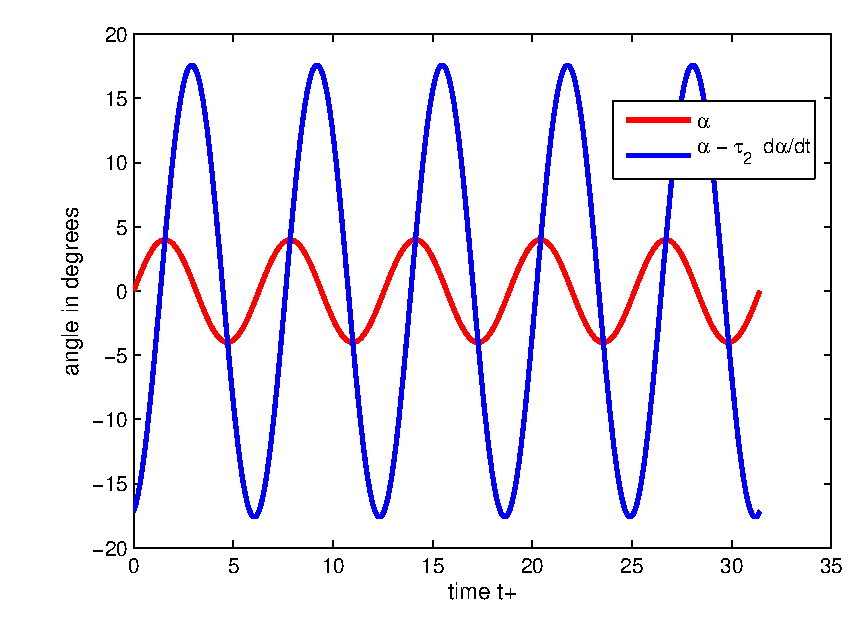
\includegraphics{./Figures/alpha_dalpha_sin_amp=4_k=0p5.eps}
  \caption{Effects of $\tau_2 \dot{\alpha}$ for high pitching rate}
  \label{fig:alpha_dalpha_vs_t}
\end{figure}


\begin{figure}[h]
  \centering
  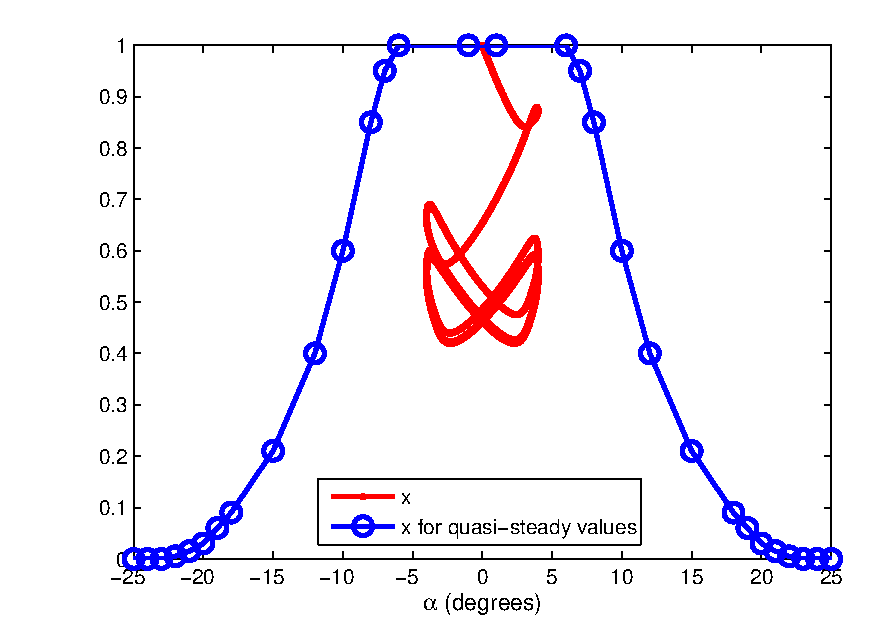
\includegraphics{./Figures/x_sin_amp=4_k=0p5.eps}
  \caption{State variable during fast sinusoidal pitching}
  \label{fig:x_fast_pitching}
\end{figure}

\par The state variable value starts at the quasi-steady value (as designed in the algorithm implementation) but after a couple of cycles it orbits close to an average value that would correspond to separated flows in a quasi-steady case.
This also leads to lower lift overall (see figure \ref{fig:Cl_fast_pitching}) since the value of x is smaller.

\begin{figure}[h]
  \centering
  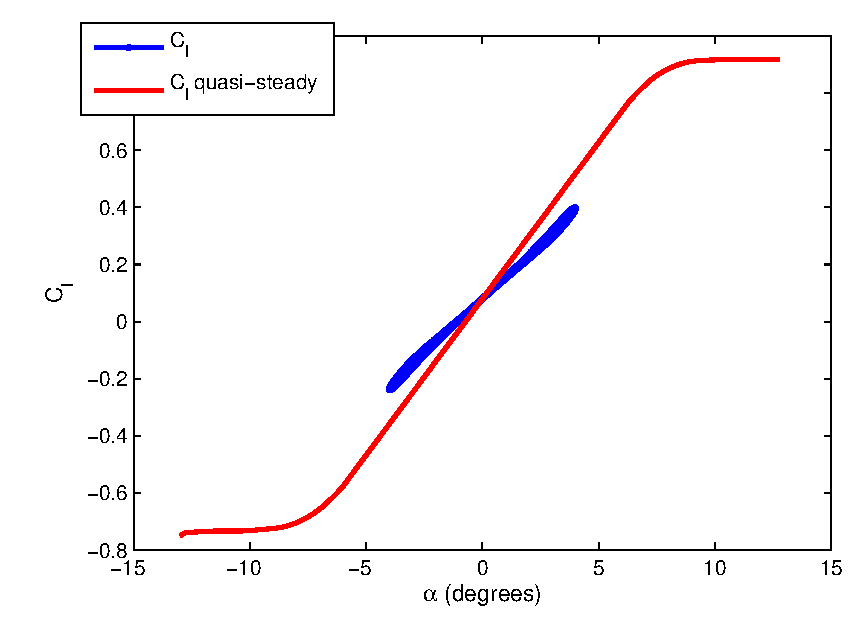
\includegraphics{./Figures/Cl_vs_alpha_amp=4_k=0p5.eps}
  \caption{$C_l$ is decreased compared to quasi-steady values for high pitching rate maneuvers (the transient part has been removed for clarity)}
  \label{fig:Cl_fast_pitching}
\end{figure}

\par If the exact same constraints are used for optimization then the problem is  illustrated by figure \ref{fig:unlimited_alpha_dot}.	

\begin{figure}[h]
  \begin{center}
  
<++>%\includegraphics{<+file+>}
\end{center}
  \caption{Optimization for vertical wind gusts with the same constraints as the previous cases}
  \label{fig:unlimited_alpha_dot}
\end{figure}

The issue is that the in order to reach the favorable high lift regions the algorithm producesm

%Since the lift to drag ratio of the NACA0009 is about 10 (compared to 13 for the notional UAV) direct comparisons with the results presented in part \ref{sec:results_QS} are impossible.
\Subsection{The ``staircase'' optimization issue}
The pitch rate dependent effects add a lot of complexity to the optimization problem.
One of the biggest is that to keep a reasonably low execution time for the optimization, the number of points has to be kept relatively low (less than a hundred).
Such discretization of the interval can cause issues in the discrete integration parts of the algorithm.
It seems that for most optimization cases this effect is avoided.

\par However the results of the of optimization for short gusts ($0.2<T_g<0.5$) sometime shows a ``staircase'' pattern in the angle of attack.

\begin{figure}[h]
  \centering
  %\includegraphics{<+file+>}
  \caption{Staircase pattern seen for XXXX wind gust with $T_g=XX$}
  \label{fig:staircase_case}
\end{figure}

\par In those cases the algorithm attempts to ``game'' the GK model with this jerky pitch motion.
Our theory is that this jerky motion avoids the decrease of the lift coefficient caused by high pitch rates by doing those for only short amount of time.
These spikes in the pitch rate are too short to be able to influence the low pass equation regulating the value of $x$.

\Section{A closer look at the high performing short gusts}

\begin{figure}[h]
  \begin{center}
  \scalebox{1.0}{
    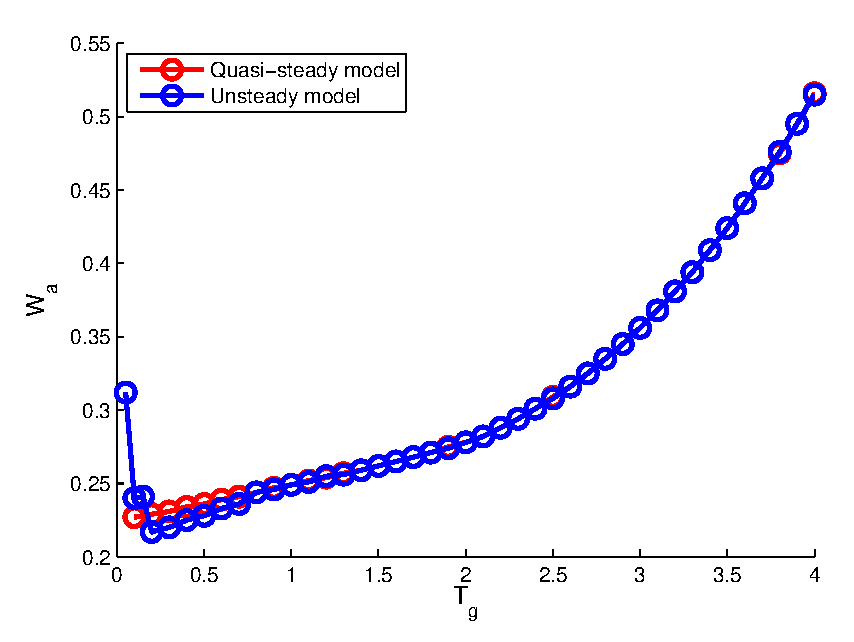
\includegraphics{./Figures/LUT_vs_GK_Wg_vs_TG_windtype=3_alhpamax=12_nodalphalimit.eps}}
  \end{center}
  \caption{Performance difference between quasi-steady and unsteady model for combined gusts}
  \label{fig:WG_vs_TG_wt=3}
\end{figure}


\begin{figure}[h]
  \centering
  \scalebox{1.0}{
    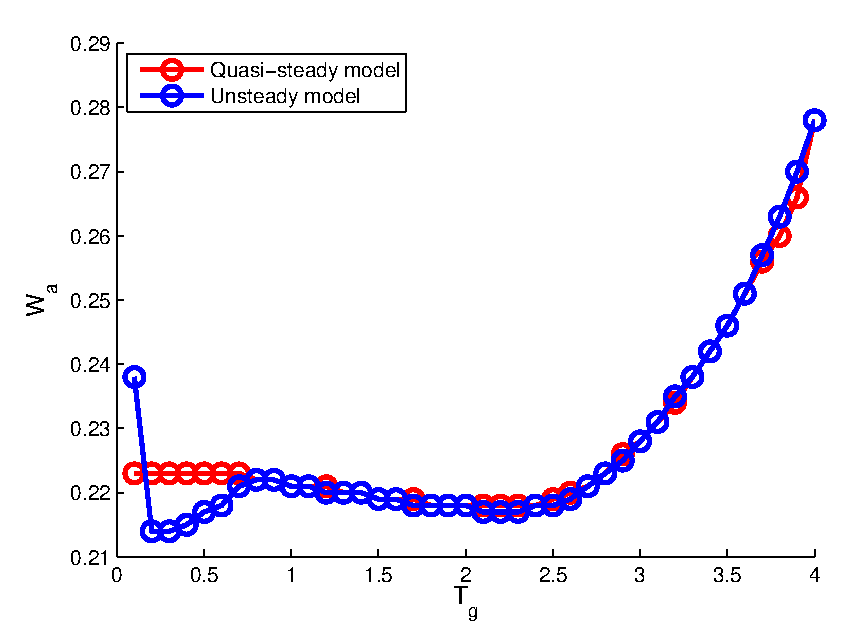
\includegraphics{./Figures/LUT_vs_GK_Wg_vs_TG_windtype=1_alhpamax=12_nodalphalimit.eps}}
  \caption{Performance difference between quasi-steady and unsteady model for vertical gusts}
  \label{fig:WG_vs_TG_wt=1}
\end{figure}

\par The difference between the quasi-steady model and the unsteady one only appears close for $T_g<0.7$.
This result is reassuring as it confirms that for long gusts ($T_g>0.7$ or $k<0.05$) the two models are equivalent.
We can confirm that there are no unsteady effects active by looking at the $C_l$ versus $\alpha$ curve compared to the quasi-steady map, or even better $G$ the lift to drag ratio.
On figure \ref{fig:G_vs_alpha_wt=1_Tg=1_GK.eps} it can be seen that the lift to drag ratio for $T_g=1$ is following the quasi-steady values.

\begin{figure}[h]
  \centering
  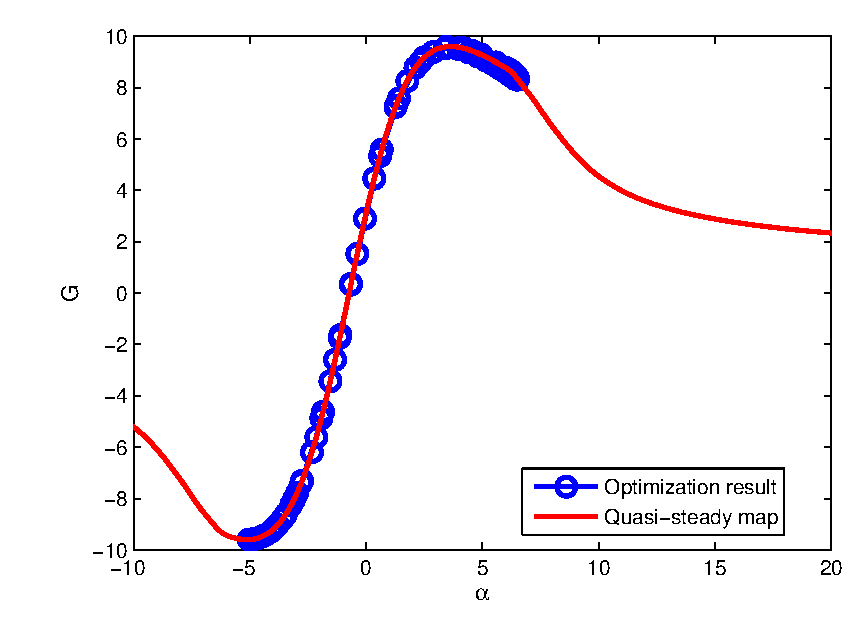
\includegraphics{./Figures/G_vs_alpha_wt=1_Tg=1_GK.eps}
  \caption{Lift to drag ratio for the unsteady model, vertical wind gust and gust duration of 1T}
  \label{fig:G_vs_alpha_wt=1_Tg=1_GK.eps}
\end{figure}

\par However for shorter gusts the results are more interesting.
We can see that for shorter gusts ($T_g<0.7$) the performances are better with the GK model than with the quasi-steady model.
This is true for both vertical and combined wind gusts, which indicates that this is due to the unsteady effects starting to be significant at this frequency.

\FloatBarrier

\par Looking more closely at the results around $T_g=0.3$, we try to highlight the differences between the quasi-steady and the unsteady model.
First we can look at the optimization parameter $\alpha$ for both vertical and combined gusts.

\begin{figure}[h]
  \centering
  \scalebox{1.0}{
    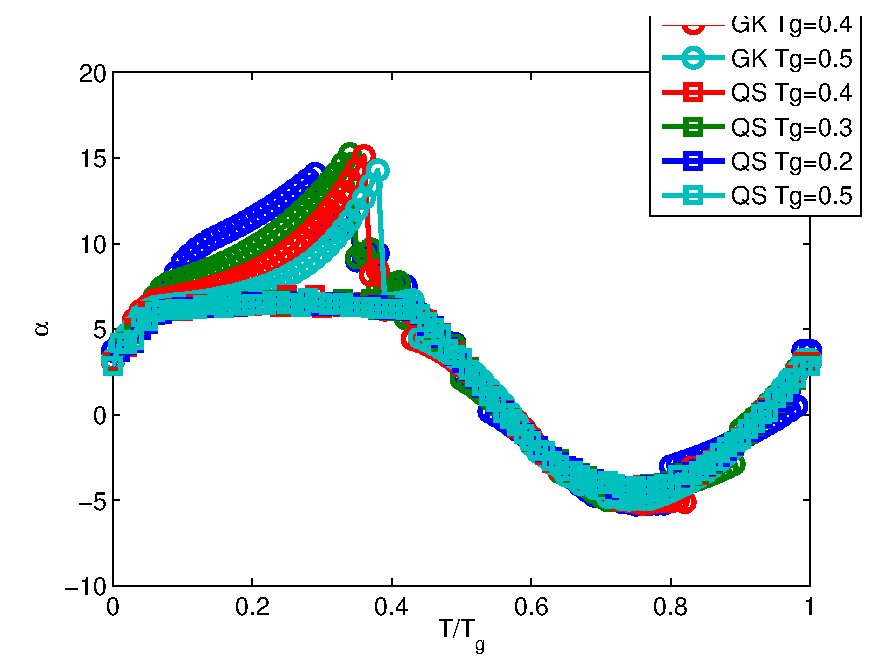
\includegraphics{./Figures/alpha_vs_Tg_wt1.eps}}
  \caption{Angle of attack for short vertical gusts with the quasi-steady (QS) and unsteady (GK) model}
  \label{fig:alpha_vs_Tg_wt1}
\end{figure}

\begin{figure}[h]
  \centering
  \scalebox{1.0}{
    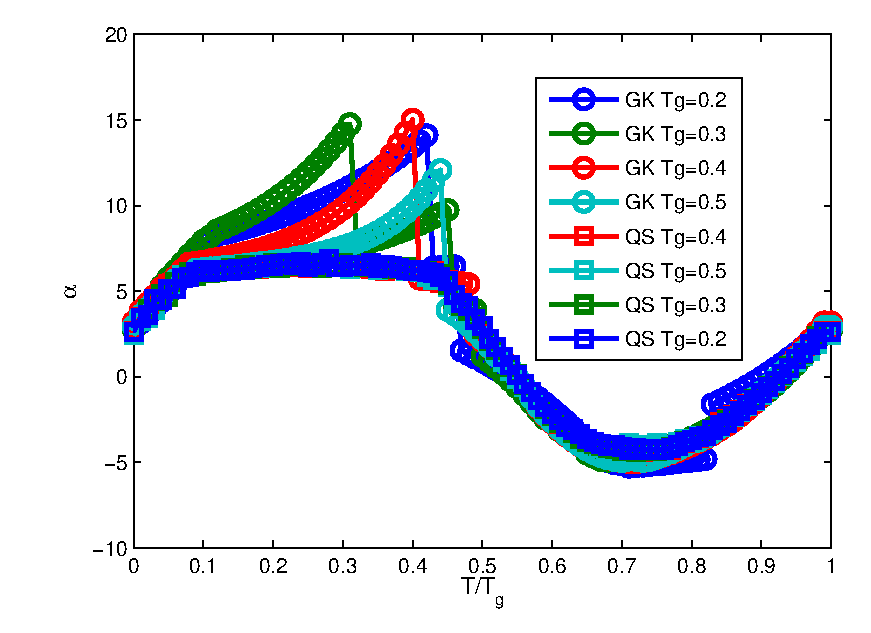
\includegraphics{./Figures/alpha_vs_Tg_wt3.eps}}
  \caption{Angle of attack for short combined gusts with the quasi-steady (QS) and unsteady (GK) model}
  \label{fig:alpha_vs_Tg_wt3}
\end{figure}

\par It is immediately apparent that the main difference is in the high angle of attack area.
Alpha increases exponentially before a sharp decrease happens around 30 to 40\% of the gust duration.
The angle of attack then falls back to the quasi-steady values.

\FloatBarrier

\par To understand what happens to the lift when such a maneuver is performed we have to refer to the lift coefficient versus angle of attack plot.

\begin{figure}[h]
  \centering
  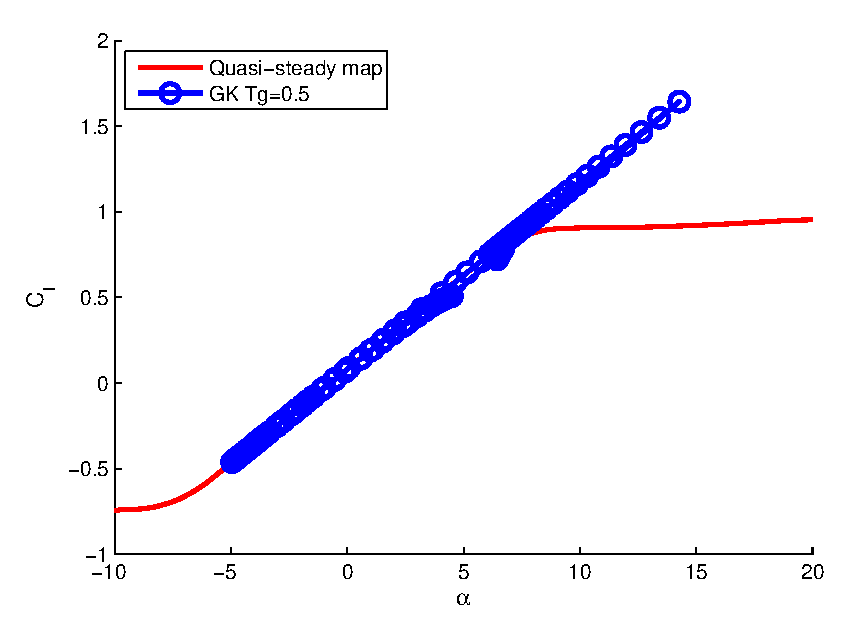
\includegraphics{./Figures/Cl_vs_alpha_wt=1_tg=0p5_alphamax=20.eps}
  \caption{Lift coefficient versus angle of attack for 0.5T long vertical wind gusts with the unsteady model}
  \label{fig:Cl_vs_alpha_short_gust_unsteady}
\end{figure}
\FloatBarrier

\par Figure \ref{fig:Cl_vs_alpha_short_gust_unsteady} illustrates perfectly the effects of the unsteady aerodynamic model and the difference with the quasi-steady model.
The spiking in angle of attack allows the flow to remain attached to the airfoil, and lets the lift coefficient reach values much higher than the quasi-steady (red curve) model would ever permit.
Sharply decreasing the angle of attack at the end of this maneuver means that the flow doesn't have time to separate.
Similar results are observed for vertical and horizontal gusts in the $T_g=0.2$ to $0.7$ region.

\Section{Bad performance at $T_g\leq0.1$}

\par As seen on figures \ref{fig:WG_vs_TG_wt=3} and \ref{fig:WG_vs_TG_wt=1} while the unsteady model optimizations are showing a more efficient energy extraction than the quasi-steady for $0.2 \leq T_g \leq 0.7$ it is not the case at $T_g=0.1$. 


\Section{Limitations of the unsteady GK model}

\Subsection{Considering the gusting and plunging component}
One of the major issues with this optimization is that it misses are the unsteady effects due to gusting and plunging.
In our case we have major gusts present at the same time as the pitching motion.
While the speed of the UAV changes too, the relative wind amplitude is in the order of 20\%.
We know that gusts as gentle as 5\% of the free stream speed can have a large influence on the lift characteristics, and that the lift response to such gusts depends strongly on the frequency of the gusts.
The same can be said for the plunging motion.

\par While these variations in $C_l$ are large it is suspected that they are caused by the same kind of mechanism as the lift variations caused by pitch angle changes.
With that in mind there is a fairly high probability that the resulting mechanism could be described by a model inspired by the GK model.
It is very likely that the state variable for such a model would be tied in some way to the state variable presented in this thesis.
If $x$ could be expressed as a function of $\alpha$, $\dot{\alpha}$ and $\dot{u}$ (for example), this model could be applicable to a whole new range of situations.

